

\documentclass[11pt,compress,t,notes=noshow, xcolor=table]{beamer}
\usepackage[]{graphicx}\usepackage[]{color}
% maxwidth is the original width if it is less than linewidth
% otherwise use linewidth (to make sure the graphics do not exceed the margin)
\makeatletter
\def\maxwidth{ %
  \ifdim\Gin@nat@width>\linewidth
    \linewidth
  \else
    \Gin@nat@width
  \fi
}
\makeatother

\definecolor{fgcolor}{rgb}{0.345, 0.345, 0.345}
\newcommand{\hlnum}[1]{\textcolor[rgb]{0.686,0.059,0.569}{#1}}%
\newcommand{\hlstr}[1]{\textcolor[rgb]{0.192,0.494,0.8}{#1}}%
\newcommand{\hlcom}[1]{\textcolor[rgb]{0.678,0.584,0.686}{\textit{#1}}}%
\newcommand{\hlopt}[1]{\textcolor[rgb]{0,0,0}{#1}}%
\newcommand{\hlstd}[1]{\textcolor[rgb]{0.345,0.345,0.345}{#1}}%
\newcommand{\hlkwa}[1]{\textcolor[rgb]{0.161,0.373,0.58}{\textbf{#1}}}%
\newcommand{\hlkwb}[1]{\textcolor[rgb]{0.69,0.353,0.396}{#1}}%
\newcommand{\hlkwc}[1]{\textcolor[rgb]{0.333,0.667,0.333}{#1}}%
\newcommand{\hlkwd}[1]{\textcolor[rgb]{0.737,0.353,0.396}{\textbf{#1}}}%
\let\hlipl\hlkwb

\usepackage{framed}
\makeatletter
\newenvironment{kframe}{%
 \def\at@end@of@kframe{}%
 \ifinner\ifhmode%
  \def\at@end@of@kframe{\end{minipage}}%
  \begin{minipage}{\columnwidth}%
 \fi\fi%
 \def\FrameCommand##1{\hskip\@totalleftmargin \hskip-\fboxsep
 \colorbox{shadecolor}{##1}\hskip-\fboxsep
     % There is no \\@totalrightmargin, so:
     \hskip-\linewidth \hskip-\@totalleftmargin \hskip\columnwidth}%
 \MakeFramed {\advance\hsize-\width
   \@totalleftmargin\z@ \linewidth\hsize
   \@setminipage}}%
 {\par\unskip\endMakeFramed%
 \at@end@of@kframe}
\makeatother

\definecolor{shadecolor}{rgb}{.97, .97, .97}
\definecolor{messagecolor}{rgb}{0, 0, 0}
\definecolor{warningcolor}{rgb}{1, 0, 1}
\definecolor{errorcolor}{rgb}{1, 0, 0}
\newenvironment{knitrout}{}{} % an empty environment to be redefined in TeX

\usepackage{alltt}
\newcommand{\SweaveOpts}[1]{}  % do not interfere with LaTeX
\newcommand{\SweaveInput}[1]{} % because they are not real TeX commands
\newcommand{\Sexpr}[1]{}       % will only be parsed by R
\newcommand{\xmark}{\ding{55}}%


\usepackage[english]{babel}
\usepackage[utf8]{inputenc}

\usepackage{dsfont}
\usepackage{verbatim}
\usepackage{amsmath}
\usepackage{amsfonts}
\usepackage{amssymb}
\usepackage{bm}
\usepackage{csquotes}
\usepackage{multirow}
\usepackage{longtable}
\usepackage{booktabs}
\usepackage{enumerate}
\usepackage[absolute,overlay]{textpos}
\usepackage{psfrag}
\usepackage{algorithm}
\usepackage{algpseudocode}
\usepackage{eqnarray}
\usepackage{arydshln}
\usepackage{tabularx}
\usepackage{placeins}
\usepackage{tikz}
\usepackage{setspace}
\usepackage{colortbl}
\usepackage{mathtools}
\usepackage{wrapfig}
\usepackage{bm}
\usepackage{amsmath}
\usepackage{pifont}
\usepackage{xcolor} %colored math symbols

\usetikzlibrary{shapes,arrows,automata,positioning,calc,chains,trees, shadows}
\tikzset{
  %Define standard arrow tip
  >=stealth',
  %Define style for boxes
  punkt/.style={
    rectangle,
    rounded corners,
    draw=black, very thick,
    text width=6.5em,
    minimum height=2em,
    text centered},
  % Define arrow style
  pil/.style={
    ->,
    thick,
    shorten <=2pt,
    shorten >=2pt,}
}

\usepackage{subfig}

% Defines macros and environments
\usepackage{../../style/lmu-lecture}


\let\code=\texttt
\let\proglang=\textsf

\setkeys{Gin}{width=0.9\textwidth}

\setbeamertemplate{frametitle}{\expandafter\uppercase\expandafter\insertframetitle}

\usepackage{bbm}
% basic latex stuff
\newcommand{\pkg}[1]{{\fontseries{b}\selectfont #1}} %fontstyle for R packages
\newcommand{\lz}{\vspace{0.5cm}} %vertical space
\newcommand{\dlz}{\vspace{1cm}} %double vertical space
\newcommand{\oneliner}[1] % Oneliner for important statements
{\begin{block}{}\begin{center}\begin{Large}#1\end{Large}\end{center}\end{block}}


%new environments
\newenvironment{vbframe}  %frame with breaks and verbatim
{
 \begin{frame}[containsverbatim,allowframebreaks]
}
{
\end{frame}
}

\newenvironment{vframe}  %frame with verbatim without breaks (to avoid numbering one slided frames)
{
 \begin{frame}[containsverbatim]
}
{
\end{frame}
}

\newenvironment{blocki}[1]   % itemize block
{
 \begin{block}{#1}\begin{itemize}
}
{
\end{itemize}\end{block}
}

\newenvironment{fragileframe}[2]{  %fragile frame with framebreaks
\begin{frame}[allowframebreaks, fragile, environment = fragileframe]
\frametitle{#1}
#2}
{\end{frame}}


\newcommand{\myframe}[2]{  %short for frame with framebreaks
\begin{frame}[allowframebreaks]
\frametitle{#1}
#2
\end{frame}}

\newcommand{\remark}[1]{
  \textbf{Remark:} #1
}


\newenvironment{deleteframe}
{
\begingroup
\usebackgroundtemplate{
\includegraphics[width=\paperwidth,height=\paperheight]{../style/color/red.png}}
 \begin{frame}
}
{
\end{frame}
\endgroup
}
\newenvironment{simplifyframe}
{
\begingroup
\usebackgroundtemplate{
\includegraphics[width=\paperwidth,height=\paperheight]{../style/color/yellow.png}}
 \begin{frame}
}
{
\end{frame}
\endgroup
}\newenvironment{draftframe}
{
\begingroup
\usebackgroundtemplate{
\includegraphics[width=\paperwidth,height=\paperheight]{../style/color/green.jpg}}
 \begin{frame}
}
{
\end{frame}
\endgroup
}
% https://tex.stackexchange.com/a/261480: textcolor that works in mathmode
\makeatletter
\renewcommand*{\@textcolor}[3]{%
  \protect\leavevmode
  \begingroup
    \color#1{#2}#3%
  \endgroup
}
\makeatother


\input{../../latex-math/basic-math}
\input{../../latex-math/basic-ml}
\input{../../latex-math/ml-nn}

\newcommand{\titlefigure}{figure/backpropagation_rnn.png}
%modify picture
\newcommand{\learninggoals}{
  \item Backpropagation
  \item Exploding and Vanishing Gradients
}

\title{Deep Learning}
\date{}



\begin{document}

\lecturechapter{Recurrent Neural Networks - Backpropogation}
\lecture{I2DL}

%%%%%%%%%%%%%%%%%%%%%%%%%%%%%%%%%%%%%%%%%%%%%%%%%%%%%%%%%%%%%%%%%%
%%%%%%%%%%%%%%%%%%%%%%%%%%%%%%%%%%%%%%%%%%%%%%%%%%%%%%%%%%%%%%%%%%


%%%%%%%%%%%%%%%%%%%%%%%%%%%%%%%%%%%%%%%%%%%%%%%%%%%%%%%%%%%%%%%%%%
%%%%%%%%%%%%%%%%%%%%%%%%%%%%%%%%%%%%%%%%%%%%%%%%%%%%%%%%%%%%%%%%%%

\frame{

\frametitle{Backpropagation through time}

  \center
  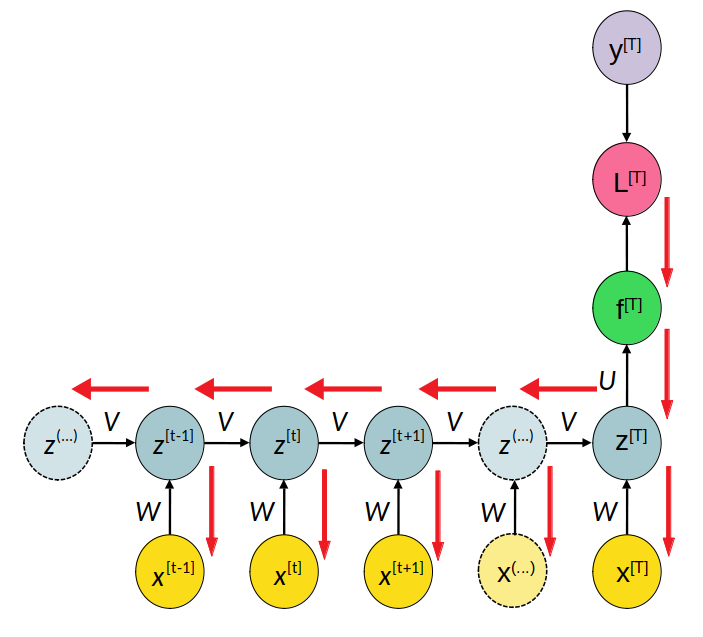
\includegraphics[width=6cm]{figure/backpropagation_rnn.png}

  %\begin{itemize}

    %\item For training the RNN we need to compute $\frac{d L}{d u_{i,j}}$, $\frac{d L}{d v_{i,j}}$, and $\frac{d L}{d w_{i,j}}$.
    %\item To do so, during backpropagation at time step $t$ %for an arbitrary RNN, 
    %we may need to compute
    $$\frac{d L}{d \bm{z}^{[1]}} = \frac{d L}{d \bm{z}^{[t]}} \frac{d \bm{z}^{[t]}}{d \bm{z}^{[t-1]}} \dots \frac{d \bm{z}^{[2]}}{d \bm{z}^{[1]}}$$

  %\end{itemize}

}


%%%%%%%%%%%%%%%%%%%%%%%%%%%%%%%%%%%%%%%%%%%%%%%%%%%%%%%%%%%%%%%%%%
%%%%%%%%%%%%%%%%%%%%%%%%%%%%%%%%%%%%%%%%%%%%%%%%%%%%%%%%%%%%%%%%%%
% \begin{vbframe}{Nlp - Example}
%       Example: 
%   \begin{itemize}
%     \item Suppose we only had a vocabulary of four possible letters: \enquote{h}, \enquote{e}, \enquote{l} and \enquote{o}
%     \item We want to train an RNN on the training sequence \enquote{hello}.
%     \item This training sequence is in fact a source of 4 separate training examples:
%       \begin{itemize}
%         \item The probability of \enquote{e} should be likely given the context of \enquote{h}
%         \item \enquote{l} should be likely in the context of \enquote{he}
%         \item \enquote{l} should also be likely given the context of \enquote{hel}
%         \item and \enquote{o} should be likely given the context of \enquote{hell}
%       \end{itemize}
%   \end{itemize}
% \end{vbframe}
%%%%%%%%%%%%%%%%%%%%%%%%%%%%%%%%%%%%%%%%%%%%%%%%%%%%%%%%%%%%%%%%%%
%%%%%%%%%%%%%%%%%%%%%%%%%%%%%%%%%%%%%%%%%%%%%%%%%%%%%%%%%%%%%%%%%%
% \frame{
% 
% \frametitle{Nlp - Example}
% 
% The RNN has a 4-dimensional input and output. The exemplary hidden layer consists of 3 neurons. This diagram shows the activations in the forward pass when the RNN is fed the characters \enquote{hell} as input. The output contains confidences the RNN assigns for the next character.
%   \begin{itemize}
%     \item[]
%   \end{itemize}
%   \begin{minipage}{0.55\textwidth}
%     \begin{figure}
%         \only<1>{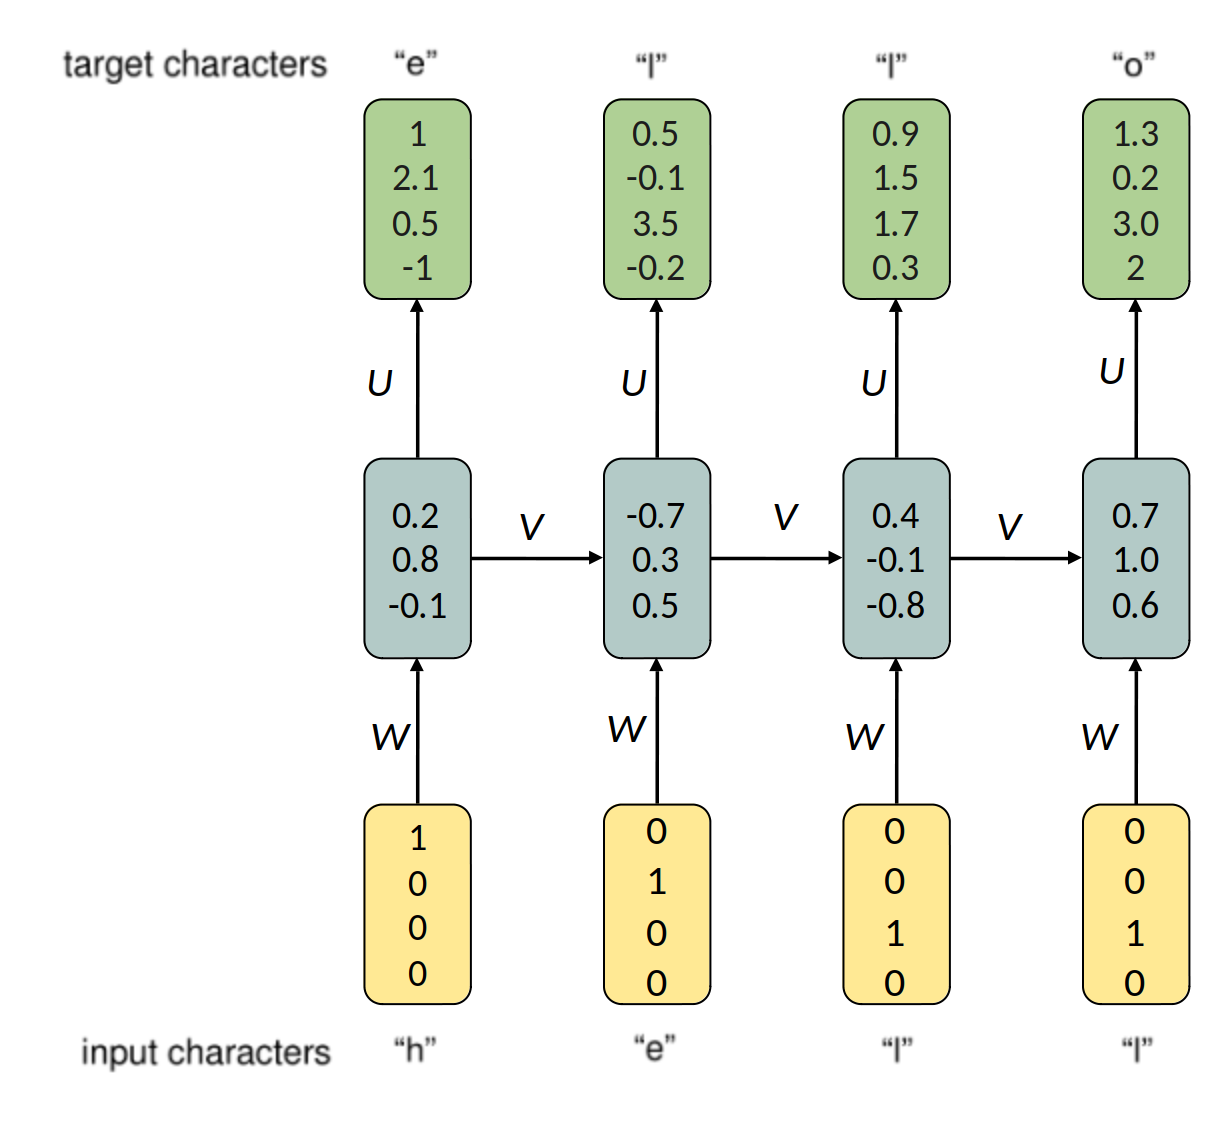
\includegraphics[width=5.5cm]{plots/nlp1.png}}%
%         \only<2>{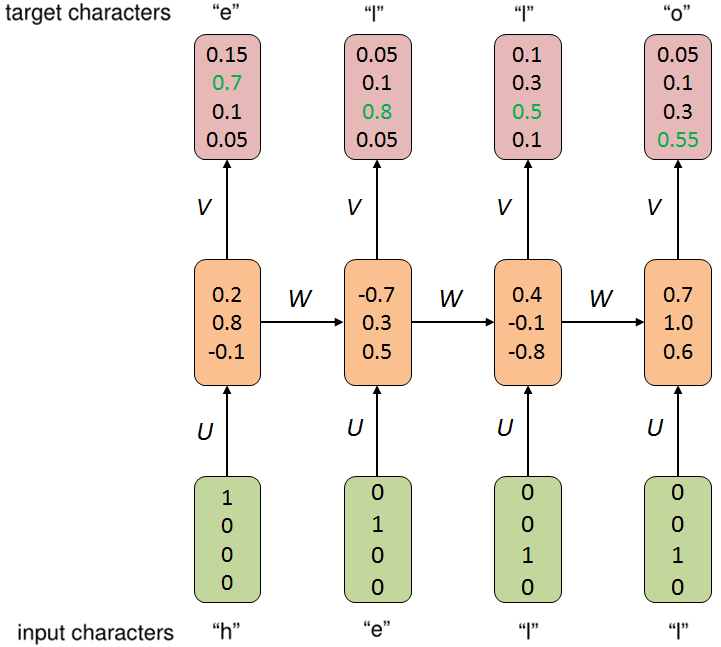
\includegraphics[width=5.5cm]{plots/nlp2.png}}%
%     \end{figure}
%   \end{minipage}%\hfill
%   \begin{minipage}{0.45\textwidth}
%   %\vspace{-0.3cm}
%   
%     \begin{itemize}
%       \only<1>{\item[] \textcolor{white}{Our goal is to increase the confidence for the correct letters (green digits) and decrease the confidence of all others (we could also use a softmax activation to squash the digits to probabilities $\in [0,1]$).}} 
%       \only<2>{\item[] Our goal is to increase the confidence for the correct letters (green digits) and decrease the confidence of all others (we could also use a softmax activation to squash the digits to probabilities $\in [0,1]$).} 
%     \end{itemize}
%   \end{minipage}
%   
% }
%%%%%%%%%%%%%%%%%%%%%%%%%%%%%%%%%%%%%%%%%%%%%%%%%%%%%%%%%%%%%%%%%%
%%%%%%%%%%%%%%%%%%%%%%%%%%%%%%%%%%%%%%%%%%%%%%%%%%%%%%%%%%%%%%%%%%
% \begin{vbframe}{Word Embeddings (Word2vec)}
%   \begin{minipage}{0.4\textwidth}
%     \begin{itemize}
%       \item Data Sparsity: 
%       \item[]
%       $$\text{man} \to \begin{bmatrix}
%                                   0\\
%                                   \vdots\\
%                                   0\\
%                                   1\\
%                                   0\\
%                                   \vdots\\
%                                   0
%                         \end{bmatrix} \to
%                         \begin{bmatrix}
%                                   0.35\\
%                                   -0.83\\
%                                   \vdots\\
%                                   0.11\\
%                                   3.2
%                         \end{bmatrix}
%       $$
%   
%     \end{itemize}
%   \end{minipage}
%   \begin{minipage}{0.55\textwidth}
%     \begin{itemize}
%       \item[]
%     \end{itemize}
%     \begin{figure}
%       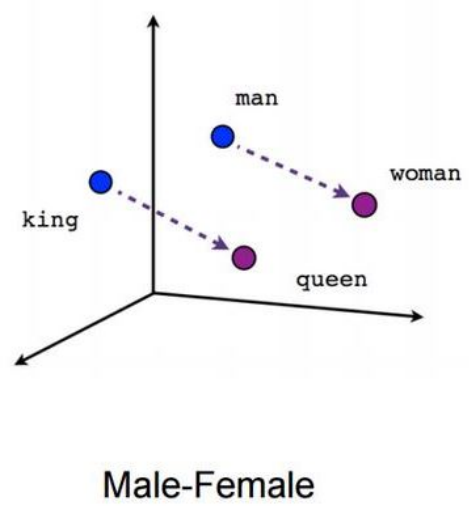
\includegraphics[width=4.5cm]{plots/word2vec.png}%
%       \caption*{https://www.tensorflow.org/tutorials/word2vec/}
%     \end{figure}    
%   \end{minipage}
% \end{vbframe}
%%%%%%%%%%%%%%%%%%%%%%%%%%%%%%%%%%%%%%%%%%%%%%%%%%%%%%%%%%%%%%%%%%
%%%%%%%%%%%%%%%%%%%%%%%%%%%%%%%%%%%%%%%%%%%%%%%%%%%%%%%%%%%%%%%%%%
\begin{vbframe}{Long-Term Dependencies}
  
  \begin{itemize}
    \item Here, $\bm{z}^{[t]} = \sigma(\bm{V}^\top \bm{z}^{[t-1]} + \bm{W}^\top \xv^{[t]} + \bm{b})$
    \item It follows that:
    $$ \frac{d \bm{z}^{[t]}}{d\bm{z}^{[t-1]}} = \text{diag}(\sigma' (\bm{V}^\top \bm{z}^{[t-1]} + \bm{W}^\top \xv^{[t]} + \bm{b})) \bm{V}^\top = \bm{D}^{[t-1]} \bm{V}^\top $$
    $$ \frac{d \bm{z}^{[t-1]}}{d\bm{z}^{[t-2]}} = \text{diag}(\sigma' (\bm{V}^\top \bm{z}^{[t-2]} + \bm{W}^\top \xv^{[t-1]} + \bm{b})) \bm{V}^\top= \bm{D}^{[t-2]} \bm{V}^\top $$
    $$ \vdots $$
    $$ \frac{d \bm{z}^{[2]}}{d\bm{z}^{[1]}} = \text{diag}(\sigma' (\bm{V}^\top \bm{z}^{[1]} + \bm{W}^\top \xv^{[2]} + \bm{b})) \bm{V}^\top = \bm{D}^{[1]} \bm{V}^\top $$
    
    $$ \frac{d L}{d \bm{z}¸^{[1]}} = \frac{d L}{d \bm{z}^{[t]}} \frac{d \bm{z}^{[t]}}{d \bm{z}^{[t-1]}} \dots \frac{d \bm{z}^{[2]}}{d \bm{z}^{[1]}} = \bm{D}^{[t-1]} \bm{D}^{[t-2]}   \text{ . . . } \bm{D}^{[1]} (\bm{V}^\top)^{t-1}$$
%    $$ \frac{d \bm{z}^{[1]}}{d\bm{x}^{[1]}} = \text{diag}(\sigma' (\bm{V}^\top \bm{z}^{[0]} + \bm{W}^\top \xv^{[1]} + \bm{b})) \bm{W}^\top$$
    \item Therefore, for an arbitrary time-step $i$ in the past, $\frac{d\bm{z}^{[t]}}{d\bm{z}^{[i]}}$ will contain the term $(\bm{V}^\top)^{t-i}$ within it (this follows from the chain rule).
    \item Based on the largest eigenvalue of $\bm{V}^\top$, the presence of the term $(\bm{V}^\top)^{t-i}$ can either result in vanishing or exploding gradients.
    \item This problem is quite severe for RNNs (as compared to feedforward networks) because the \textbf{same} matrix $\bm{V}^\top$ is multiplied several times. \href{https://tinyurl.com/vangrad}{\beamergotobutton{Click here}}
    \item As the gap between $t$ and $i$ increases, the instability worsens.
    \item It is quite challenging for RNNs to learn long-term dependencies. The gradients either \textbf{vanish} (most of the time) or \textbf{explode} (rarely, but with much damage to the optimization).
    \item That happens simply because we propagate errors over very many stages backwards.
  \end{itemize}
  
  \framebreak
  \begin{figure}
      \centering
      \scalebox{0.8}{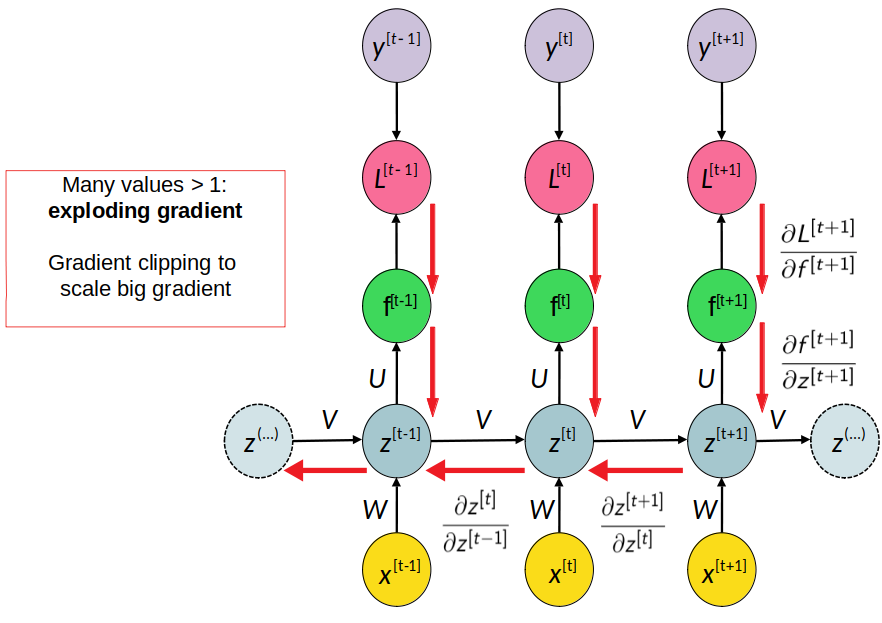
\includegraphics{figure/rnn_exploding.png}}
      \caption{\footnotesize {Exploding gradients}}
  \end{figure}

  \begin{itemize}
    \item Recall, that we can counteract exploding gradients by implementing gradient clipping.
    \item To avoid exploding gradients, we simply clip the norm of the gradient at some threshold $h$ (see chapter 4): $$\text{if  } ||\nabla W|| > \text h: \nabla W \leftarrow \frac{h}{||\nabla W||} \nabla W $$
  \end{itemize}

\framebreak

  \begin{figure}
      \centering
      \scalebox{0.8}{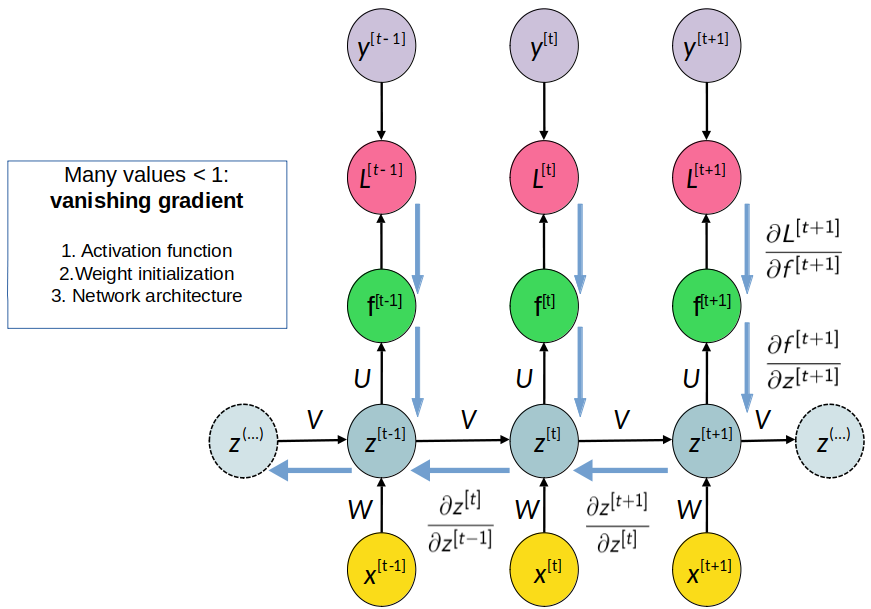
\includegraphics{figure/rnn_vanishing.png}}
      \caption{\footnotesize {Vanishing gradients}}
  \end{figure}


  \begin{itemize}
    \item Even if we assume that the parameters are such that the recurrent network is stable (can store memories, with gradients not exploding), the difficulty with long-term dependencies arises from the exponentially smaller weights given to long-term interactions (involving the multiplication of many Jacobians) compared to short-term ones.
    \item A more sophisticated solution is needed for the vanishing gradient problem in RNNs.
    \item The \textbf{vanishing gradient problem} is heavily dependent on the parameter initialization method, but in particular on the choice of the activation functions.
    \begin{itemize}
      \item For example, the sigmoid maps a real number into a \enquote{small} range (i.e. $[0, 1]$).
      \item As a result, large regions of the input space are mapped into a very small range.
      \item Even a huge change in the input will only produce a small change in the output. Hence, the gradient will be small.
      \item This becomes even worse when we stack multiple layers of such non-linearities on top of each other (For instance, the first layer maps a large input to a smaller output region, which will be mapped to an even smaller region by the second layer, which will be mapped to an even smaller region by the third layer and so on..).
      \item We can avoid this problem by using activation functions which do not have the property of \enquote{squashing} the input.
      \item The most popular choice is obviously the Rectified Linear Unit (ReLU) which maps $x$ to $max(0,x)$.
      \item The really nice thing about ReLU is that the gradient is either $0$ or $1$, which means it never saturates. Thus, gradients can't vanish.
      \item The downside of this is that we can obtain a \enquote{dead} ReLU. It will always return $0$  and consequently never learn because the gradient is not passed through.
    \end{itemize}
  \end{itemize}


\end{vbframe}
%%%%%%%%%%%%%%%%%%%%%%%%%%%%%%%%%%%%%%%%%%%%%%%%%%%%%%%%%%%%%%%%%%
%%%%%%%%%%%%%%%%%%          REFERENCES          %%%%%%%%%%%%%%%%%%
%%%%%%%%%%%%%%%%%%%%%%%%%%%%%%%%%%%%%%%%%%%%%%%%%%%%%%%%%%%%%%%%%%
\begin{vbframe}
\frametitle{References}
\footnotesize{
\begin{thebibliography}{99}
%%%%%%%%%%%%%%%%%%%%%%%%%%%%%%%%%%
\bibitem[Ian Goodfellow et al., 2016]{1} Ian Goodfellow, Yoshua Bengio and Aaron Courville (2016)
\newblock Deep Learning
\newblock \emph{\url{http://www.deeplearningbook.org/}}
%%%%%%%%%%%%%%%%%%%%%%%%%%%%%%%%%%
\bibitem[Andrej Karpathy., 2015]{1} Andrej Karpathy (2015)
\newblock The Unreasonable Effectiveness of Recurrent Neural Networks
\newblock \emph{\url{http://karpathy.github.io/2015/05/21/rnn-effectiveness/}}
%%%%%%%%%%%%%%%%%%%%%%%%%%%%%%%%%%
\end{thebibliography}
}
\end{vbframe}
%%%%%%%%%%%%%%%%%%%%%%%%%%%%%%%%%%%%%%%%%%%%%%%%%%%%%%%%%%%%%%%%%%
%%%%%%%%%%%%%%%%%%%%%%%%%%%%%%%%%%%%%%%%%%%%%%%%%%%%%%%%%%%%%%%%%%

\endlecture
\end{document}